\newpage % Rozdziały zaczynamy od nowej strony.
\section{Dataset}

Deep learning research on medical knowledge graphs currently leaves two related
 gaps unaddressed. First, causal modeling is rarely applied at the level of 
 the full patient trajectory.
 Second, most knowledge graphs encode relationships extracted from literature, 
 without integrating patient-level empirical data on how outcomes are actually 
 observed (as well noted by \textcite{toonsi2025causal}). 
 To address both gaps, we generated a synthetic dataset that jointly 
 encodes a known causal structure and its patient-level empirical realizations, 
 providing ground truth for both link prediction and node classification. 
 This gave a full control over how knowledge is encoded in the graph, 
 avoiding reconstruction from a partially observed real-world dataset.
 The generation process, the resulting graph, and the derived patient data are 
 described in detail in this chapter. 
 
 Additionally, there is included 
 a description of benchmark datasets used for testing the prototyped models.

\subsection{Synthethic dataset}

The dataset includes two structures:

\begin{enumerate}
    \item a causal knowledge graph (DAG) that encodes causal patient pathways
    from patient characteristics and drug exposures to clinical events
    (endpoints);
    \item an empirical dataset --- a patient-level table with each patient's
    characteristics and observations, generated from the knowledge graph
    (Section~\ref{subsec:generation}).
\end{enumerate}

\subsubsection{Knowledge graph}

The construction of the knowledge graph started from defining the clinical
endpoints to model and predict, and identifying which patient
characteristics and drug exposures are known to influence them. This
approach -- starting from the target and working backwards to its
determinants -- was chosen so that every path in the graph corresponds to a
patient clinical pathway.

As our team includes a team member with a pharmacology background, her
domain knowledge was used for constructing and verifying the initial version
of the knowledge graph -- the first set of endpoints, risk factors, and
drug classes. Candidate mechanistic pathways connecting a drug exposure to a
given endpoint, including specific drug-drug and drug-disease interaction
gates, were proposed with the support of
Fable\footnote{Fable refers to Claude Fable 5, a large language model
developed by Anthropic, which was used as an AI-assisted modelling aid to
draft candidate mechanistic pathways for review.}. All proposals generated
with its support were accepted, rejected, or modified by the team member
with a pharmacology background before being incorporated into the graph
specification.

The graph was built iteratively. An initial, smaller version of the DAG
covered a limited set of drug classes, 
mechanisms, and endpoints. Once this core structure was
validated, it was progressively extended with
additional nodes and edges. The final version includes 155 nodes organised
into six layers specified in Tables ~\ref{tab:node_types} and 405 directed edges grouped into categories in 
~\ref{tab:edge_type_categories}.

\begin{table}[htbp]
    \centering
    \caption{Node types in the patient causal DAG.}
    \label{tab:node_types}
    \begin{tabularx}{\textwidth}{@{}l X@{}}
        \toprule
        \textbf{Node type} & \textbf{Description} \\
        \midrule
        \texttt{patient\_context} & Patient-level covariates (e.g. demographics, comorbidities). \\
        \addlinespace
        \texttt{drug\_exposure} & Drugs the patient is exposed to. \\
        \addlinespace
        \texttt{mechanism} & Intermediate physiological mechanisms mediating the effect of a drug or context on further stages. \\
        \addlinespace
        \texttt{adr\_or\_intermediate\_state} & Intermediate adverse or physiological states positioned between mechanisms and clinical endpoints. \\
        \addlinespace
        \texttt{observation\_or\_selection} & Nodes representing observation, documentation, or selection processes rather. \\
        \addlinespace
        \texttt{clinical\_endpoint} & Target adverse clinical outcomes (e.g. AKI, DILI, Hospitalization). \\
        \bottomrule
    \end{tabularx}
\end{table}


\begin{figure}[h]
    \centering
    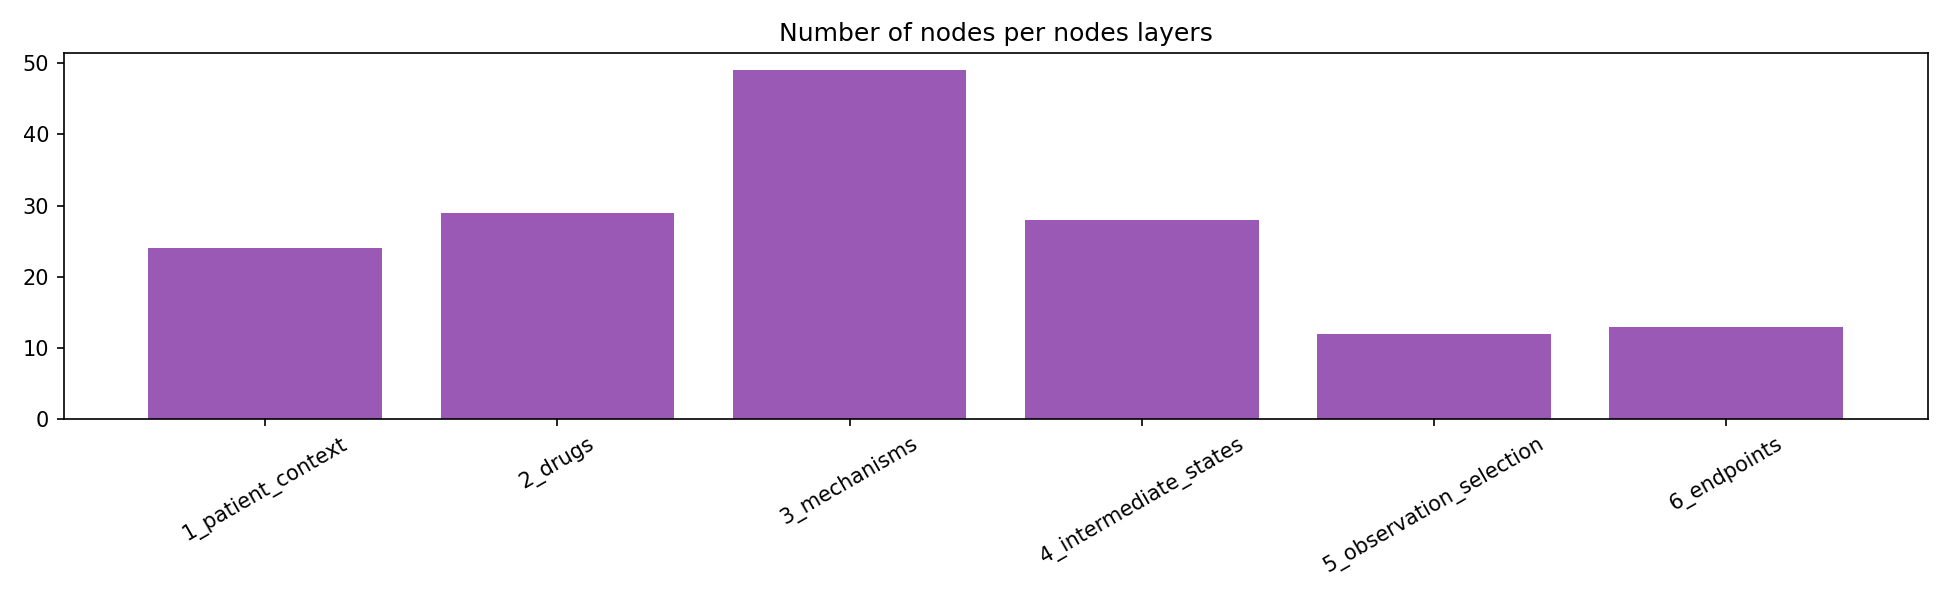
\includegraphics[width=\textwidth, height=0.45\textheight, keepaspectratio]{rysunki/01_node_counts_by_type_and_layer.png}
    \caption{Frequency of nodes types.}
    \label{fig:architecture}
\end{figure}

Beyond its topology, every node in the graph carries a set of attributes
which are used directly in the
data-generating process described in Section~\ref{subsec:generation}:

\begin{itemize}
    \item \texttt{base\_prevalence} encodes a population-level
    probability of a node being present in a patient who has none of the
    node's risk factors active.
    \item \texttt{severity\_weight} encodes the clinical severity assigned to
    a node, independent of how frequently it occurs.
    \item \texttt{observability} encodes how reliably a true clinical state is
    expected to be recorded in practice.
\end{itemize}

\begin{table}[htbp]
    \centering
    \small
    \setlength{\tabcolsep}{5pt}
    \renewcommand{\arraystretch}{1.2}
    \caption{Semantic categories of directed edges in the patient causal DAG.}
    \label{tab:edge_type_categories}

    \begin{tabular}{@{}p{0.30\textwidth} p{0.64\textwidth}@{}}
        \toprule
        \textbf{Category} & \textbf{Included edge types} \\
        \midrule

        Background risk and treatment assignment &
        \makecell[l]{
            \texttt{risk\_modifier}, \texttt{confounding},\\
            \texttt{latent\_confounding}, \texttt{treatment\_indication},\\
            \texttt{treatment\_burden}
        } \\
        \addlinespace[3pt]

        Drug effects and mechanistic pathways &
        \makecell[l]{
            \texttt{drug\_to\_mechanism}, \texttt{causal\_mechanistic},\\
            \texttt{mechanism\_to\_adr}, \texttt{adr\_to\_intermediate}
        } \\
        \addlinespace[3pt]

        Clinical outcome progression &
        \makecell[l]{
            \texttt{adr\_to\_endpoint},\\
            \texttt{endpoint\_to\_hospitalization}
        } \\
        \addlinespace[3pt]

        Observation and selection processes &
        \makecell[l]{
            \texttt{observation}, \texttt{selection},\\
            \texttt{observation\_process}
        } \\
        \addlinespace[3pt]

        Polypharmacy, aggregate burden, and interactions &
        \makecell[l]{
            \texttt{drug\_to\_burden}, \texttt{drug\_to\_load},\\
            \texttt{interaction\_gate\_component},\\
            \texttt{drug\_pairwise\_gate}, \texttt{drug\_triple\_gate},\\
            \texttt{interaction\_amplify},\\
            \texttt{adr\_burden\_component}, \texttt{burden\_threshold}
        } \\
        \bottomrule
    \end{tabular}
\end{table}

As edges bring different information based on edge type, they were assigned declared attributes, such as:

\begin{itemize}
    \item \texttt{effect\_size} encodes the strength of the causal effect of
    the source node on the target node.
    \item \texttt{effect\_sign} encodes the direction of that effect
    (risk-increasing or risk-decreasing).
\end{itemize}

In \cref{fig:dag_overview} it is visualized an overview of DAG graph. 

\begin{figure}[h]
    \centering
    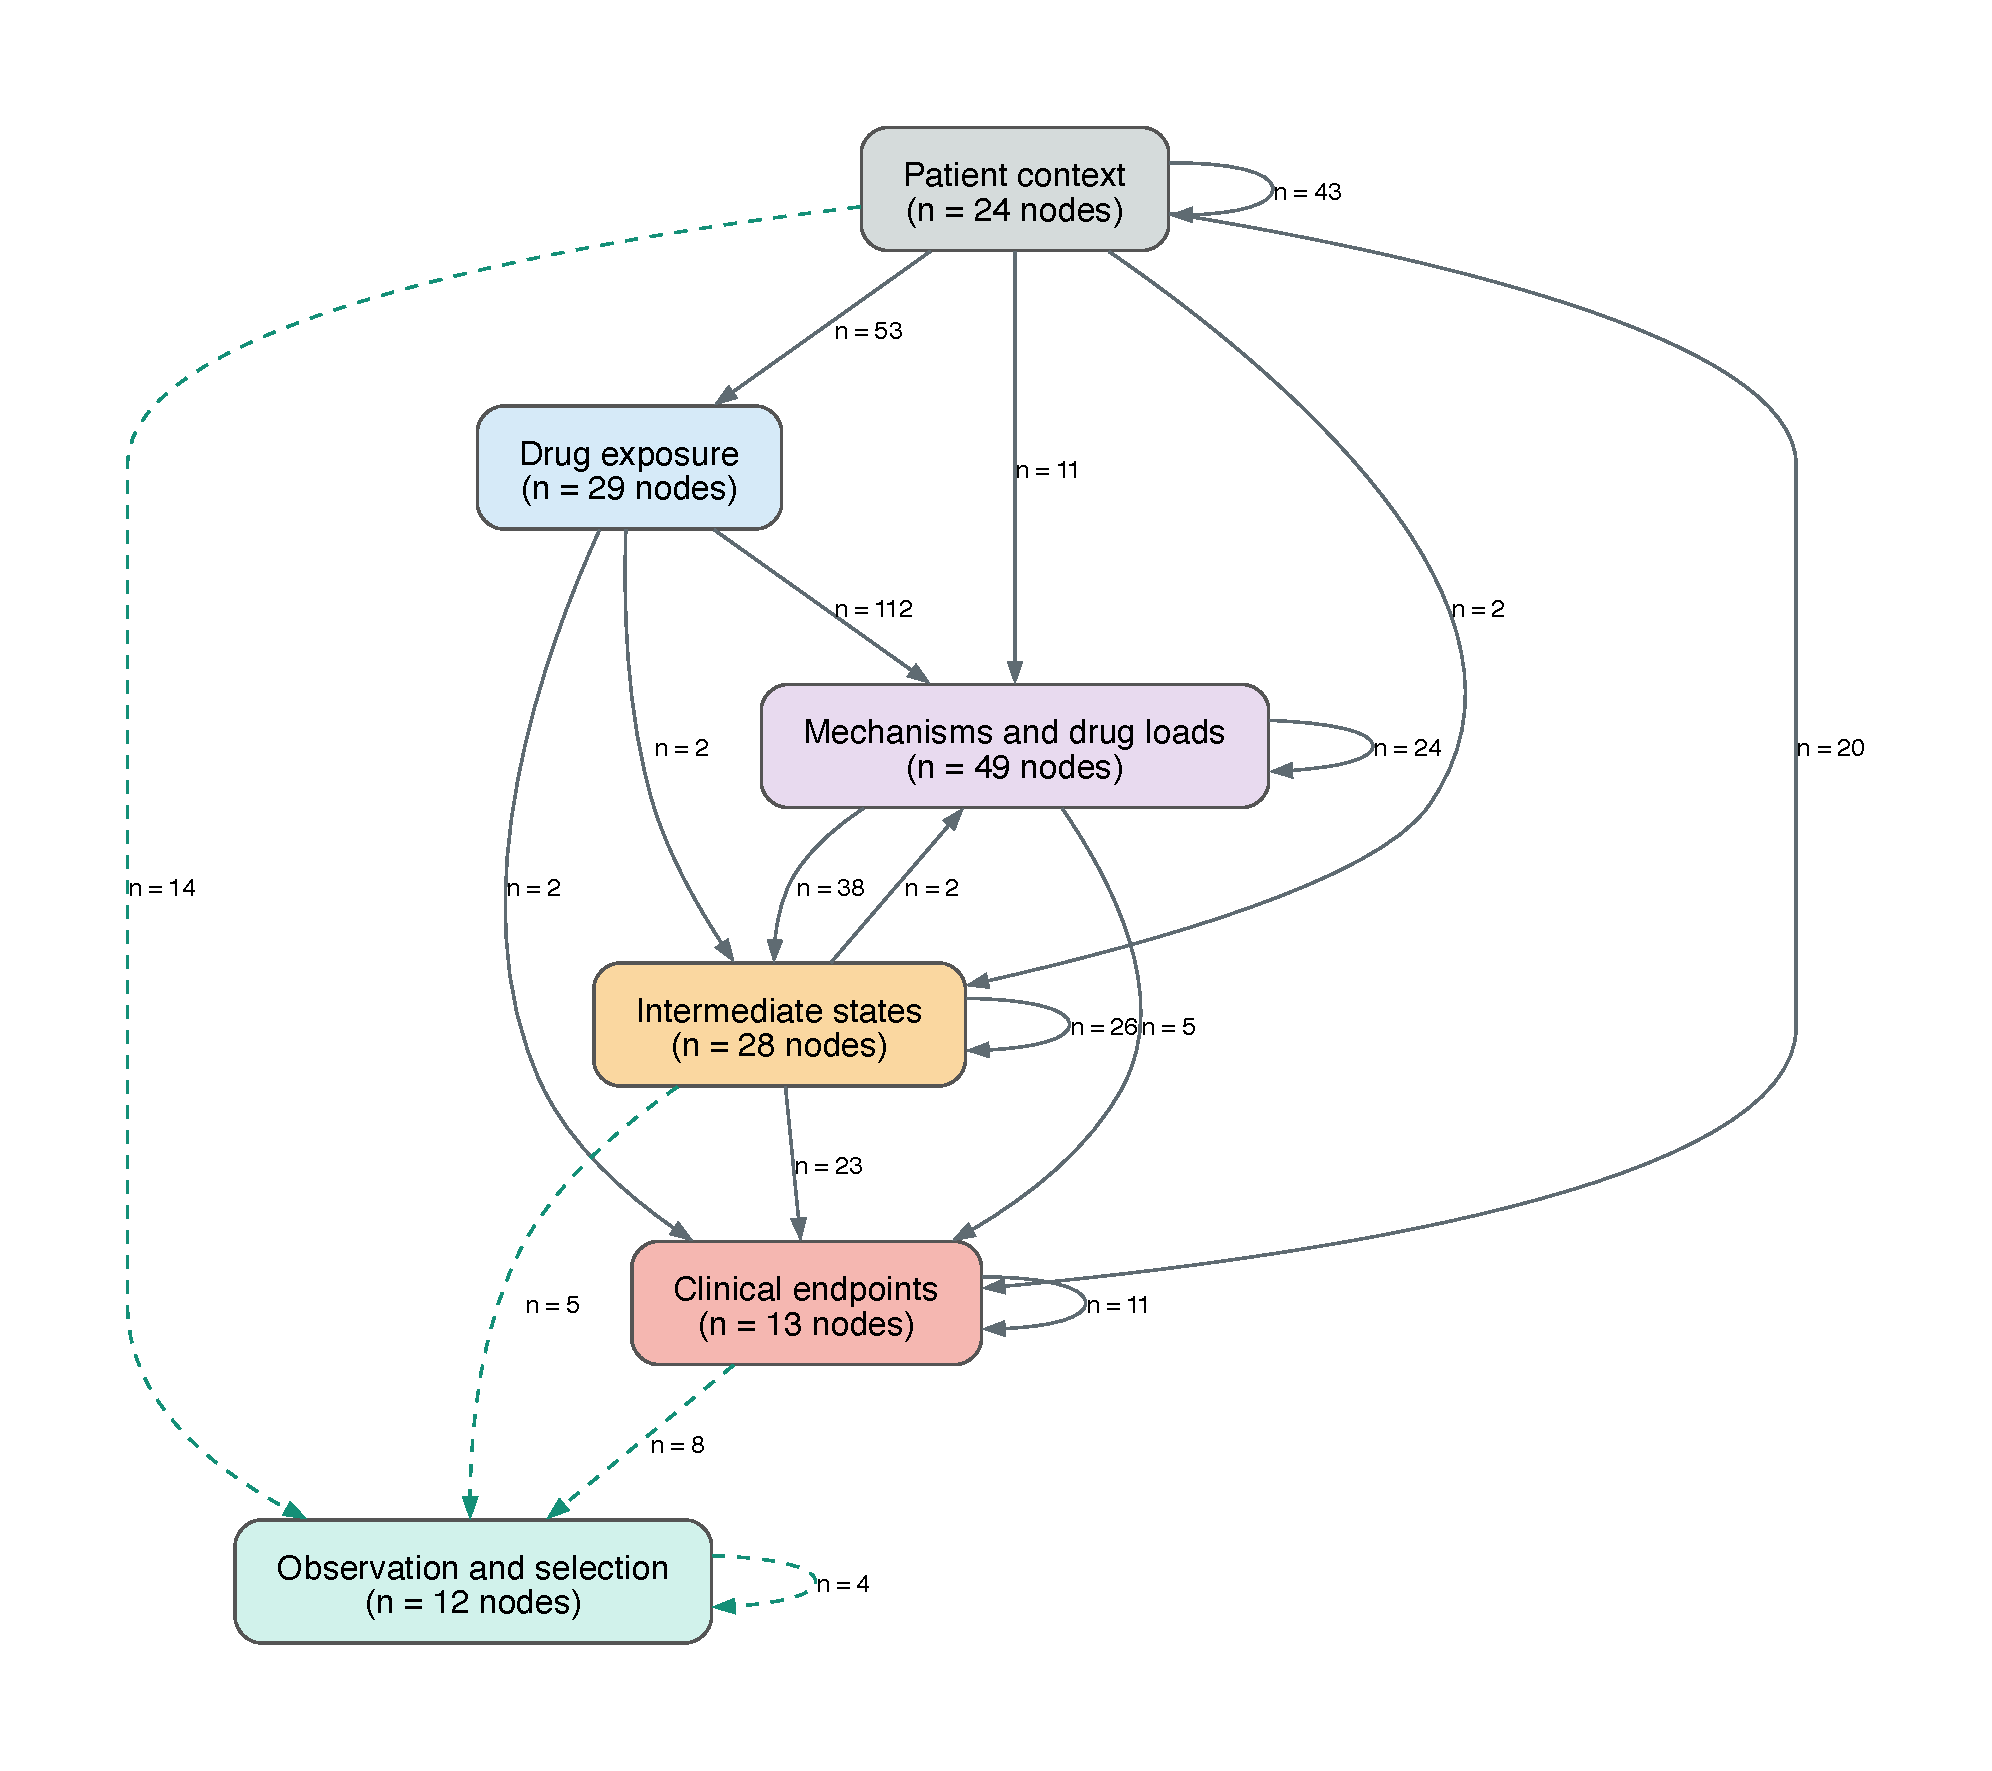
\includegraphics[width=\textwidth, height=0.45\textheight, keepaspectratio]{rysunki/causal_dag_type_overview.pdf}
    \caption{DAG visualization}
    \label{fig:dag_overview}
\end{figure}

The final version of the DAG was verified statistically with the metrics
reported in \cref{tab:dag_structural_stats}. They confirm the graph's
acyclicity and characterize its structural complexity for modelling
purposes.

\begin{table}[htbp]
    \centering
    \caption{Structural statistics of the causal knowledge graph.}
    \label{tab:dag_structural_stats}
    \begin{tabularx}{\textwidth}{@{}l X@{}}
        \toprule
        \textbf{Metric} & \textbf{Value} \\
        \midrule
        Nodes / edges & 155 / 405 \\
        Graph density & 0.017 \\
        Acyclicity  & True \\
        Self-loops / duplicate edges & 0 / 0 \\
        Source nodes / sink nodes & 9 / 12 \\
        Direct parents per clinical endpoint & mean 4.7 (range 1--14) \\
        Ancestors per clinical endpoint & median 31 (range 9--126) \\
        Longest root-to-endpoint path & median 12 edges (range 5--16) \\
        Shortest root-to-endpoint path & 1 edge for 10 of 13 endpoints; 3--4 edges for the three rarest endpoints \\
        %Causal motifs (mediation / fork / collider) & 922 / 1{,}545 / 1{,}022 triplets \\
        Drug--endpoint pairs sharing a common ancestor & 85 \\
        \bottomrule
    \end{tabularx}
\end{table}

% It is worth to mention that DAG includes 
% an unobserved confounder \texttt{unobserved\_severity} that accounts for 741 of the
% 1{,}545 fork triplets in the graph (48\%) -- that's why it is recommended for exclusion
% on the 
%  Second, the three
% endpoints with the lowest Bayes ceiling (Section~\ref{sec:generation}) --
% serotonin syndrome, rhabdomyolysis, and lactic acidosis -- are exactly the
% three endpoints with a single direct parent and the longest minimum
% root-to-endpoint distance (3--4 edges, versus 1 edge for all other
% endpoints). This is a purely structural property, observable without
% generating a single patient, and it independently corroborates the
% distributional finding reported later in this chapter.


\subsubsection{Patient data}
\label{subsec:generation}

The patient-level data generation procedure was designed to produce
tabular records that provide empirical evidence for knowledge-graph
reconstruction and downstream prediction of clinical outcomes. Its purpose
was to transform the static causal DAG specification into a patient-level
dataset in which each individual is represented by a realised configuration
of exposures, clinical states, and outcomes. This enables the graph
representation to be used as a dynamic, data-supported structure for
multiple downstream tasks.
For each of 20{,}000 simulated patients, the generator assigns a realised
value to each of the 155 nodes in the causal DAG. Values are generated in
topological order, following the causal direction of the graph. For every
patient, upstream context variables are generated first, followed by drug
exposures, physiological mechanisms, and intermediate adverse states.
Clinical endpoints are generated only after all their parent variables have
been realised.
Each node value is generated by one of three mechanisms:
a stochastic process, a deterministic computation of other nodes, or a
deterministic observation rules. The following paragraphs
describe each mechanism.

\paragraph{Stochastic nodes}
Most nodes -- patient covariates, drug exposures, intermediate mechanisms,
and clinical endpoints -- are generated as Bernoulli draws whose probability
is a logistic function of their parents:

\begin{equation}
\eta_i = \operatorname{logit}(p_i^{0}) + \sum_{j \in \mathrm{parents}(i)} s_{ij} \cdot w_{ij} \cdot x_j,
\qquad
x_i \sim \mathrm{Bernoulli}\big(\sigma(\eta_i)\big),
\end{equation}

where $p_i^{0}$ is the node's baseline prevalence, $x_j$ is the realised
value of parent $j$, and $w_{ij}$, $s_{ij}$ are the effect size and effect
sign declared on the edge $j \to i$. Nodes are generated in topological
order, so that every parent has already been assigned a value before its
children are processed.

Three conditions affect the implementation:

\begin{itemize}
    \item A parent with more than two distinct realised values (i.e.\ a
    \texttt{count} or \texttt{continuous} node, such as
    \texttt{polypharmacy\_burden}) is standardised before entering
    the sum, $(x_j - \bar{x}_j) / \mathrm{sd}(x_j)$, so that its
    contribution to $\eta_i$ is on a comparable scale to binary parents.
    \item $p_i^{0}$ is taken from the \texttt{base\_prevalence} column of
    the node specification \footnote{If base prevalence value is missing, a type-dependent
    default is used instead (0.16 for drug exposures, 0.02 for clinical
    endpoints, 0.35 for observation/selection nodes, 0.10 otherwise)}.
    \item  If missing, \texttt{effect\_size}, and
    \texttt{effect\_sign} defaults to 0.5 and $+1$ accordingly.
\end{itemize}

\paragraph{Deterministic derived variables.}

Some variables are derived deterministically from values that have already been
generated based on  patterns of polypharmacy, drug interactions, and
adverse-event burden explicit in the graph.

Table~\ref{tab:deterministic_variables} summarises the deterministic
variables and their generating rules. 
%The complete variable-level
%data-generating specification is provided in
%Appendix~\ref{app:data_generating_spec}.

\begin{table}[htbp]
    \centering
    \small
    \caption{Deterministic variables in the synthetic patient generator.}
    \label{tab:deterministic_variables}
    \begin{tabularx}{\textwidth}{@{}
        p{0.33\textwidth}
        p{0.18\textwidth}
        X@{}}
        \toprule
        \textbf{Variable group} &
        \textbf{Rule type} &
        \textbf{Generating rule} \\
        \midrule

        Renal, CNS, bleeding, serotonergic, and hepatic
        \texttt{ddi\_*} gates &
        Conjunctive gate &
        A binary variable equal to 1 only when all listed drug-exposure
        components are active. For example,
        \texttt{ddi\_renal\_triple\_whammy}
        $= \texttt{nsaid} \land \texttt{acei\_arb} \land
        \texttt{diuretic}$. \\

        \addlinespace
        Drug--disease interaction gates
        (\texttt{drug\_disease\_*}) &
        Conjunctive gate &
        A binary variable equal to 1 when the relevant drug exposure or drug
        load and the associated patient risk factor are both active. \\

        \addlinespace
        \texttt{active\_drug\_count} &
        Drug count &
        Sum of all 29 binary \texttt{drug\_exposure} variables. \\

        \addlinespace
        Drug-load variables
        (\texttt{nephrotoxin\_load}, \texttt{hepatic\_drug\_load},
        \texttt{qt\_drug\_load\_v3}, \texttt{cns\_depressant\_load},
        \texttt{bleeding\_risk\_load}, \texttt{serotonergic\_load},
        \texttt{cyp\_inhibitor\_load}) &
        Drug count &
        Sum of active drug exposures belonging to a predefined clinical risk
        group. \\

        \addlinespace
        \texttt{ddi\_qt\_multidrug\_load} &
        Drug count &
        Sum of active QT-prolonging drug exposures specified in the
        generator. \\

        \addlinespace
        \texttt{ddi\_serotonergic\_high\_load} &
        Threshold &
        Equal to 1 when \texttt{serotonergic\_load} is at least 2. \\

        \addlinespace
        \texttt{cumulative\_adr\_burden} &
        Weighted sum &
        Severity-weighted sum of intermediate adverse states plus
        $0.08 \times \texttt{active\_drug\_count}$. \\

        \addlinespace
        \texttt{severe\_adr\_burden} &
        Threshold &
        Equal to 1 when \texttt{cumulative\_adr\_burden} is at least 4.0. \\

        \bottomrule
    \end{tabularx}
\end{table}

\paragraph{Deterministic observation rules}

A small set of variables is generated deterministically as the product of an
underlying clinical state and its associated observation process. For
example,

\[
\texttt{elevated\_creatinine\_recorded}
=
\texttt{creatinine\_rise}
\times
\texttt{creatinine\_tested}.
\]

These variables represent recorded clinical evidence rather than the
underlying patient state alone. Thus, a creatinine rise may be present but
remain absent from the recorded data if no creatinine test is performed.
Analogous deterministic rules are applied to recorded ALT/AST elevation and
recorded QT prolongation.

The observation variables distinguish clinical truth from documentation and
are retained as part of the complete data-generating process. They also
provide a structured representation of testing and recording mechanisms that
is relevant to the construction and interpretation of alternative
observational scenarios.


\subsubsection{Evaluation scenarios}



Data was generated in five controlled
scenarios constructed to evaluate model robustness under common
challenges of observational clinical data. All scenarios use the same
underlying synthetic pharmacotherapy DAG and preserve the semantic meaning of
node and edge types. Each scenario modifies either the available information,
the sampling mechanism, the treatment-assignment process, the observation
process, or the institutional context. 

For example, the \texttt{selectionbias} scenario restricts the cohort to
patients with hospital contact, creatinine testing, and liver-function
testing. Consequently, inclusion depends on downstream healthcare-contact
and diagnostic processes. The observation and documentation variables therefore support
interpretation of this scenario.

All of scenarios are presented in Table ~\ref{tab:synthethic_scenarios}.

\begin{table}[htbp]
    \centering
    \small
    \caption{Synthetic evaluation scenarios and their intended data challenge.}
    \label{tab:synthetic_scenarios}
    \begin{tabularx}{\textwidth}{@{}l X@{}}
        \toprule
        \textbf{Scenario} & \textbf{Primary purpose} \\
        \midrule
        \texttt{clean} &
        Reference setting with complete generated information. \\
        \addlinespace

        \texttt{hidden\_confounder} &
        Unmeasured confounding: \texttt{unobserved\_severity} remains active
        in the generator but is withheld from the observed data. \\
        \addlinespace

        \texttt{selection\_bias} &
        Selection bias induced by restricting the cohort to patients with
        hospital contact, creatinine testing, and liver-function testing. \\
        \addlinespace

        \texttt{no\_overlap} &
        Positivity violation caused by subgroup-specific treatment
        probabilities. \\
        \addlinespace

        \texttt{noisy\_documentation} &
        Imperfect clinical recording, including false negatives and a 1\%
        false-positive recording probability. \\
        \addlinespace

        \texttt{multihospital} &
        Institutional heterogeneity in treatment assignment and documentation
        processes across four synthetic hospitals. \\
        \bottomrule
    \end{tabularx}
\end{table}

\subsubsection{Resulting patient-level dataset}

Th final dataset generated
contains 20{,}000 simulated patients for every scenario described. Each row represents one patient and
each graph node is represented by a corresponding patient-level variable.
Table~\ref{tab:patient_dataset_schema} summarises the structure and value
types of the resulting dataset. A complete variable-level data dictionary is
provided in Appendix~\ref{appendix-list}.

\begin{table}[htbp]
    \centering
    \caption{Schema of the generated patient-level dataset.}
    \label{tab:patient_dataset_schema}
    \begin{tabularx}{\textwidth}{@{}X c X@{}}
        \toprule
        \textbf{Variable group} &
        \textbf{Number} &
        \textbf{Value type} \\
        \midrule

        \texttt{patient\_id} &
        1 &
        Integer identifier. \\

        \addlinespace
        \texttt{hospital\_id} &
        1 &
        Categorical integer identifier. \\

        \addlinespace
        \texttt{patient\_context} &
        24 &
        Mostly binary; selected count and baseline-measurement variables. \\

        \addlinespace
        \texttt{drug\_exposure} &
        29 &
        Binary. \\

        \addlinespace
        \texttt{mechanism} &
        49 &
        Binary, count, and deterministic gate variables. \\

        \addlinespace
        \texttt{adr\_or\_intermediate\_state} &
        28 &
        Mostly binary; derived score and threshold variables. \\

        \addlinespace
        \texttt{observation\_or\_selection} &
        12 &
        Binary. \\

        \addlinespace
        \texttt{clinical\_endpoint} &
        13 &
        Binary. \\

        \bottomrule
    \end{tabularx}
\end{table}

\texttt{Clinical endpoints}

The 13 clinical endpoints are binary stochastic variables generated after
their direct parents have been realised. Their values are the ground-truth
labels used for endpoint prediction. Table~\ref{tab:app_endpoints} lists the
endpoint names and their direct parents in the final DAG.

\begin{table}[htbp]
    \centering
    \small
    \caption{Endpoint prevalence and AUROC ceiling in the evaluation subset.}
    \label{tab:app_endpoints}
    \begin{tabular}{lrrrr}
        \toprule
        \textbf{Endpoint} &
        \textbf{Positive cases} &
        \textbf{Prevalence (\%)} &
        \textbf{AUROC ceiling (\%)} &
        \textbf{Parents} \\
        \midrule
        AKI                 & 393 & 13.10 & 81.13 & 6 \\
        DILI                & 55  & 1.83  & 65.29 & 7 \\
        Delirium            & 111 & 3.70  & 66.80 & 4 \\
        Depression          & 254 & 8.47  & 65.25 & 6 \\
        Falls               & 234 & 7.80  & 69.67 & 7 \\
        GI bleeding         & 64  & 2.13  & 57.04 & 5 \\
        Hospitalization     & 676 & 22.53 & 75.07 & 14 \\
        Hyperkalemia        & 146 & 4.87  & 58.98 & 2 \\
        Hyponatremia        & 236 & 7.87  & 63.83 & 3 \\
        QT arrhythmia       & 48  & 1.60  & 62.24 & 4 \\
        Serotonin syndrome  & 8   & 0.27  & 55.45 & 1 \\
        Rhabdomyolysis      & 11  & 0.37  & 53.02 & 1 \\
        Lactic acidosis     & 17  & 0.57  & 52.32 & 1 \\
        \bottomrule
    \end{tabular}
\end{table}

\paragraph{Patient-level data splits}

Patients were partitioned into mutually exclusive training, validation, and
test sets in proportions of 70\%, 15\%, and 15\%, respectively. For the
\texttt{clean} scenario containing 20{,}000 patients, this corresponds to
14{,}000 training patients, 3{,}000 validation patients, and 3{,}000 test
patients.

Splits were created at the \texttt{patient\_id} level using a deterministic
greedy multi-label balancing procedure with seed \texttt{20260722}. Patients
with rare endpoint combinations were assigned first, and assignments were
chosen to preserve the prevalence of each clinical endpoint across the three
splits. Consequently, every patient appears in exactly one split, while the
multi-label endpoint distribution remains approximately balanced.

A single master split assignment was derived from the \texttt{clean}
scenario and reused across all alternative scenarios. This ensures that
performance differences between scenarios reflect the intended changes in
data scenarios.

\subsection{Benchmark Dataset}

\subsubsection{Last-FM dataset}

\subsubsection{Hetionet knowledge graph}
\label{subsec:hetionet}

Hetionet is a heterogeneous network
(\emph{hetnet}) that integrates biomedical knowledge from 29 publicly
available resources. It represents biological and pharmacological entities
as nodes and documented relationships between them as typed edges.

Hetionet v1.0 contains 47{,}031 nodes belonging to 11 node types and
2{,}250{,}197 relationships of 24 types. The graph includes compounds,
diseases, genes, anatomies, pathways, biological processes, molecular
functions, cellular components, pharmacologic classes, side effects, and
symptoms. This heterogeneous structure makes Hetionet suitable for node classification task described further. 
The details of benchmark is included in Section ~\ref{subsec:benchmark-endpoint}.

\begin{figure}[h]
    \centering
    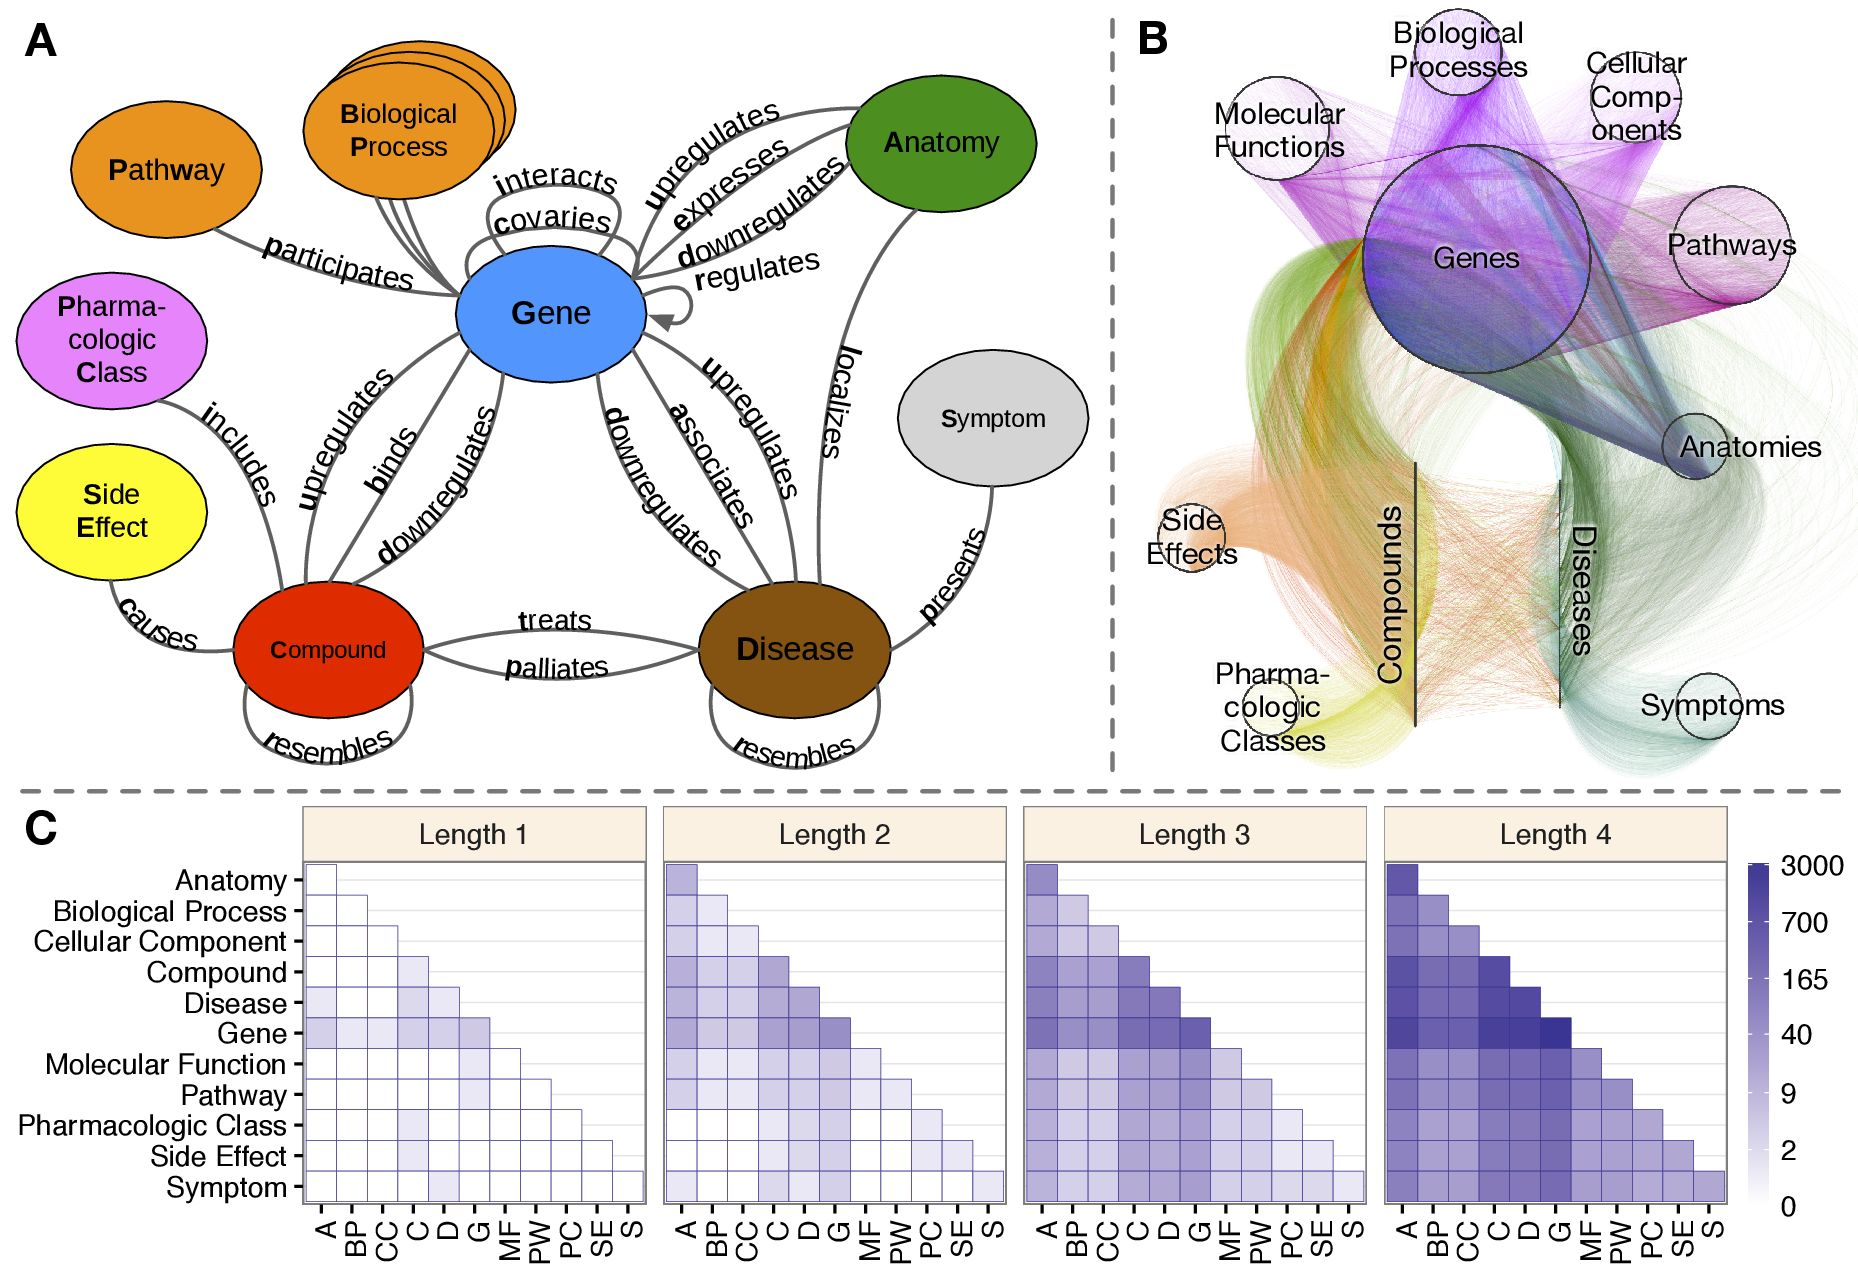
\includegraphics[width=\textwidth, height=0.45\textheight, keepaspectratio]{rysunki/elife-26726-fig1-v2.jpg}
    \caption{Hetionet knowledge graph}
    \label{fig:hetionet-original}
\end{figure}

%wstawić rysunek
%https://github.com/hetio/hetionet
%https://elifesciences.org/articles/26726/figures

